\documentclass[conference]{IEEEtran}
\usepackage[T1]{fontenc}
\usepackage{mathptmx}
\usepackage{amsmath,graphicx,booktabs,url}
\graphicspath{{../../results/phase2/study/}{../../results/phase2/hybrid/}}
\title{Card Fraud Triage via Gaussian Mixture Density and Autoencoder Reconstruction\\Phase 2: Neural Anomaly Detection}
\author{\IEEEauthorblockN{Team T085}\IEEEauthorblockA{Section E, Project 26\\Rishihood University}}
\begin{document}
\maketitle

\begin{abstract}
We compare frozen Gaussian mixture (GMM) and denoising autoencoder scores on ULB/Kaggle card transactions. We report four validation-calibrated false-positive budgets and run 12 controlled autoencoder ablations. We also fuse the two model scores on a shared empirical tail scale. Mixed validation selects a 95\% GMM and 5\% autoencoder weighting. On the previously inspected historical test, the hybrid attains 0.5754 average precision, compared with 0.5822 for GMM and 0.0908 for the autoencoder. At 284 reviews, the hybrid matches the GMM at 57 of 75 frauds.
\end{abstract}
\begin{IEEEkeywords}
card fraud, anomaly detection, autoencoder, Gaussian mixture, precision-recall
\end{IEEEkeywords}

\section{Introduction and Related Work}
A fraud review team needs a useful ranking under a fixed workload. A Gaussian mixture provides a flexible density model of legitimate transactions, but covariance estimation can be unstable with many features. Dempster et al.~\cite{dempster} provide the EM framework used to fit this model. Sakurada and Yairi~\cite{sakurada} study nonlinear reconstruction for anomaly detection. An autoencoder can learn a nonlinear representation where Phase 1 PCA reconstruction uses a linear subspace. Vincent et al.~\cite{vincent} motivate denoising by learning to reconstruct clean inputs from corrupted versions. Reconstruction error can assign similar scores to a well-reconstructed fraud and a legitimate transaction, so we judge ranking directly. Precision-recall analysis is particularly informative for rare positives~\cite{saito}.

\section{Data and Models}
The original ULB/Kaggle data~\cite{ulb} contain 284,807 transactions and 492 frauds. The frozen chronological train, validation and historical test partitions contain 170,888, 56,958 and 56,961 rows. The validation and historical test partitions contain 57 and 75 frauds. Both original model pipelines start from the same pool of 170,528 legitimate training rows. They use V1--V28 and $\log(1+\mathrm{Amount})$ with legitimate-only scaling. Time defines chronology. Class identifies legitimate training rows and provides evaluation labels.

\textbf{Frozen GMM.} The Phase 1 fit selects 20 full-covariance components by training BIC. Its anomaly score is negative log density.

\textbf{Frozen autoencoder.} A network with widths $29,16,8,16,29$ uses ReLU hidden units, a linear output and Adam with 512-row batches. The eight-unit bottleneck compresses the inputs. Gaussian noise with standard deviation 0.05 gives small perturbations on the standardized scale. The historical run generated its noisy inputs before fitting and used a random 10\% legitimate-only reserve. Scikit-learn monitored internal validation $R^2$~\cite{sklearn}. Training reached the 35-epoch cap. On clean inputs the anomaly score is
\begin{equation}
s(\mathbf{x})=\frac{1}{29}\sum_{j=1}^{29}(x_j-\hat{x}_j)^2.
\end{equation}

\section{Historical Comparison}
For each model, we sort legitimate validation scores and freeze a cutoff for each nominal FPR budget. An alert requires a score strictly above the cutoff. We report actual historical test FPR because the population and score distribution can shift. Top-$k$ policies select a fixed number of records for both models. Table~\ref{tab:rank} reports ranking metrics. Table~\ref{tab:fpr} reports false alerts and recall.

\begin{table}[t]\centering
\caption{Frozen scores on the historical test}\label{tab:rank}
\begin{tabular}{lrrrr}
\toprule
Model & AP & PR AUC & ROC AUC & P@284 \\
\midrule
GMM & 0.5822 & 0.5787 & 0.9187 & 20.07\% \\
Autoencoder & 0.0908 & 0.0885 & 0.9319 & 11.62\% \\
\bottomrule
\end{tabular}
\end{table}

\begin{table}[t]\centering
\caption{Validation budgets applied to the historical test}\label{tab:fpr}
\begin{tabular}{rrrrrrr}
\toprule
& \multicolumn{3}{c}{GMM} & \multicolumn{3}{c}{Autoencoder} \\
\cmidrule(lr){2-4}\cmidrule(lr){5-7}
Budget & Recall & FP & FPR & Recall & FP & FPR \\
\midrule
0.1\% & 73.3\% & 29 & 0.051\% & 0.0\% & 26 & 0.046\% \\
0.5\% & 76.0\% & 175 & 0.308\% & 36.0\% & 135 & 0.237\% \\
1.0\% & 77.3\% & 324 & 0.570\% & 46.7\% & 314 & 0.552\% \\
5.0\% & 80.0\% & 2082 & 3.660\% & 80.0\% & 2169 & 3.813\% \\
\bottomrule
\end{tabular}
\end{table}

\begin{figure}[t]\centering
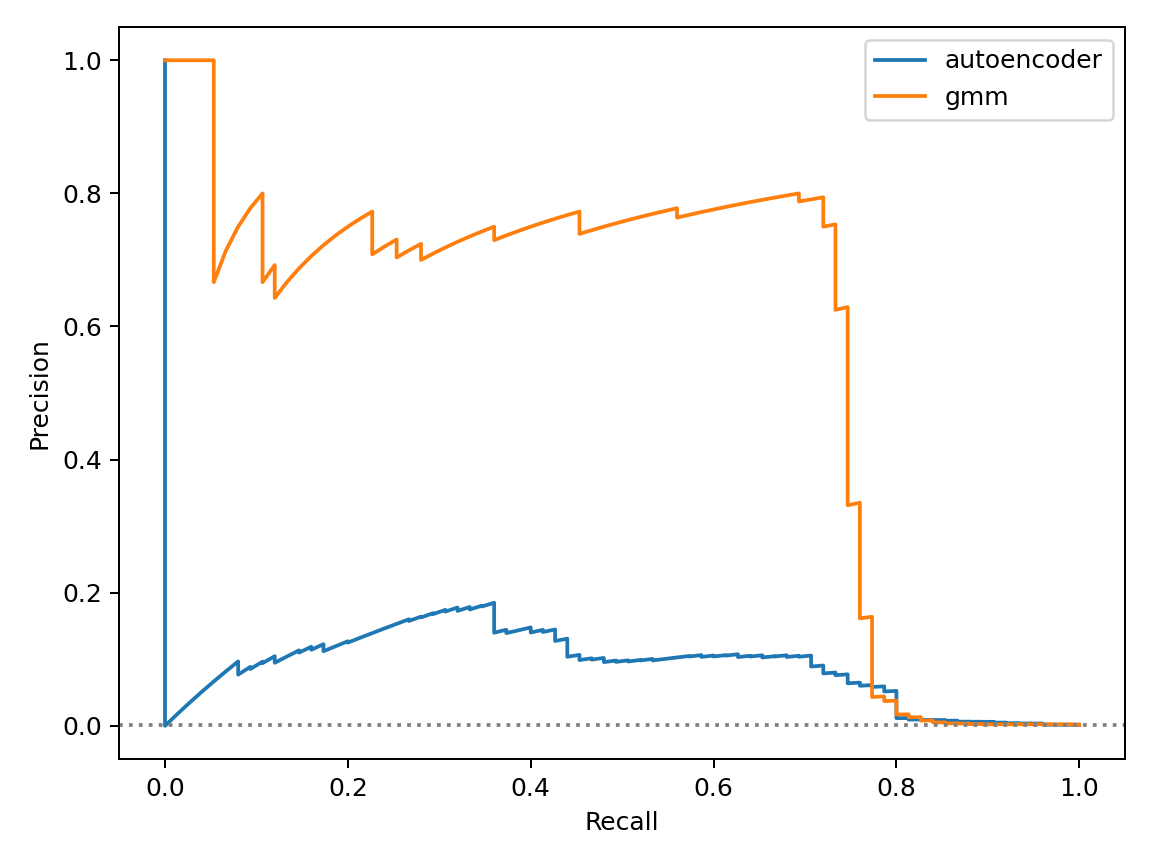
\includegraphics[width=\columnwidth]{test_pr_curve.png}
\caption{Precision-recall curves on the previously inspected historical test. The dotted line represents 0.132\% fraud prevalence.}\label{fig:pr}
\end{figure}

At the 0.5\% budget, the GMM generates 232 alerts and the autoencoder generates 162. The equal-capacity comparison fixes the effort at 284 reviews and recovers 57 frauds with GMM and 33 with the autoencoder. At 5\%, both recover 60 frauds while each generates more than 2,000 false alerts. The autoencoder's higher ROC AUC coexists with substantially lower early-queue precision (Fig.~\ref{fig:pr}).

\section{Validation-Only Ablation}
We compare widths 4, 8 and 16 with Gaussian noise of 0.05 and add a clean-input model at width 8. Seeds 13, 26 and 42 are paired across variants. The earlier 153,474 legitimate rows fit the scaler and neural weights. The later 17,054 legitimate rows form a common chronological checkpoint reserve. We keep timestamp ties together. Denoising trials draw fresh corruption each epoch. All variants use Adam with the same learning rate, batch size and L2 penalty, and select the epoch with the lowest clean reserve MSE within a 35-epoch cap and five-epoch patience. The mixed validation set measures fraud ranking after checkpoint selection. This controlled protocol is separate from the original autoencoder fit.

\begin{table}[t]\centering
\caption{Ablation on mixed validation across three seeds}\label{tab:ablation}
\begin{tabular}{rrrrr}
\toprule
Width & Noise SD & Mean AP & SD of AP & Mean recall$^*$ \\
\midrule
8 & 0.05 & 0.0497 & 0.0082 & 41.5\% \\
8 & 0.00 & 0.0507 & 0.0090 & 42.7\% \\
4 & 0.05 & 0.0491 & 0.0050 & 40.4\% \\
16 & 0.05 & 0.0606 & 0.0050 & 46.8\% \\
\bottomrule
\multicolumn{5}{l}{\footnotesize $^*$At the 0.5\% validation FPR budget.}
\end{tabular}
\end{table}

At width 8 the mean AP difference with and without noise is small relative to seed variation. Width 16 has the highest mean AP of the variants tested. The frozen GMM reaches 0.6299 AP on the same mixed validation rows. The executed notebook includes the training objective and clean reserve reconstruction curves for the ablations.

\section{Hybrid Score Fusion}
The GMM measures local density and the autoencoder measures nonlinear reconstruction. Their raw scores have different units and ranges. We use legitimate validation transactions to give both signals a common rarity scale. For model $j$ and raw score $s$, let $N_0$ be the number of legitimate validation rows and $n_j(s)$ be the number whose score is at least $s$. We compute
\begin{equation}
t_j(s)=-\log\left(\frac{1+n_j(s)}{N_0+1}\right).
\end{equation}
The smoothing keeps the score finite above the largest reference value and limits the extreme tail to the resolution supported by the sample. It can tie very extreme scores. The hybrid combines $t_{\mathrm{GMM}}$ and $t_{\mathrm{AE}}$ with weights $1-w$ and $w$. This gives an additional signal when a low-density point also reconstructs poorly. The weighted rarity score orders transactions for review.

Mixed-validation AP selects $w$ from $\{0.05,0.10,0.20,0.35,0.50\}$, preferring smaller $w$ on ties. We freeze the winning $w=0.05$ and calibrate one threshold per FPR budget using legitimate validation rows. Each standalone score serves as a component-removal baseline. All three scores use matching rows, FPR policies and review capacities.

\begin{table}[t]\centering
\caption{Hybrid and component-removal baselines}
\label{tab:hybrid}
\begin{tabular}{lrrr}
\toprule
Model & Validation AP & Historical AP & Fraud at 284 \\
\midrule
GMM & 0.6299 & 0.5822 & 57 \\
Autoencoder & 0.0380 & 0.0908 & 33 \\
Hybrid & 0.6327 & 0.5754 & 57 \\
\bottomrule
\end{tabular}
\end{table}

\begin{figure}[t]\centering
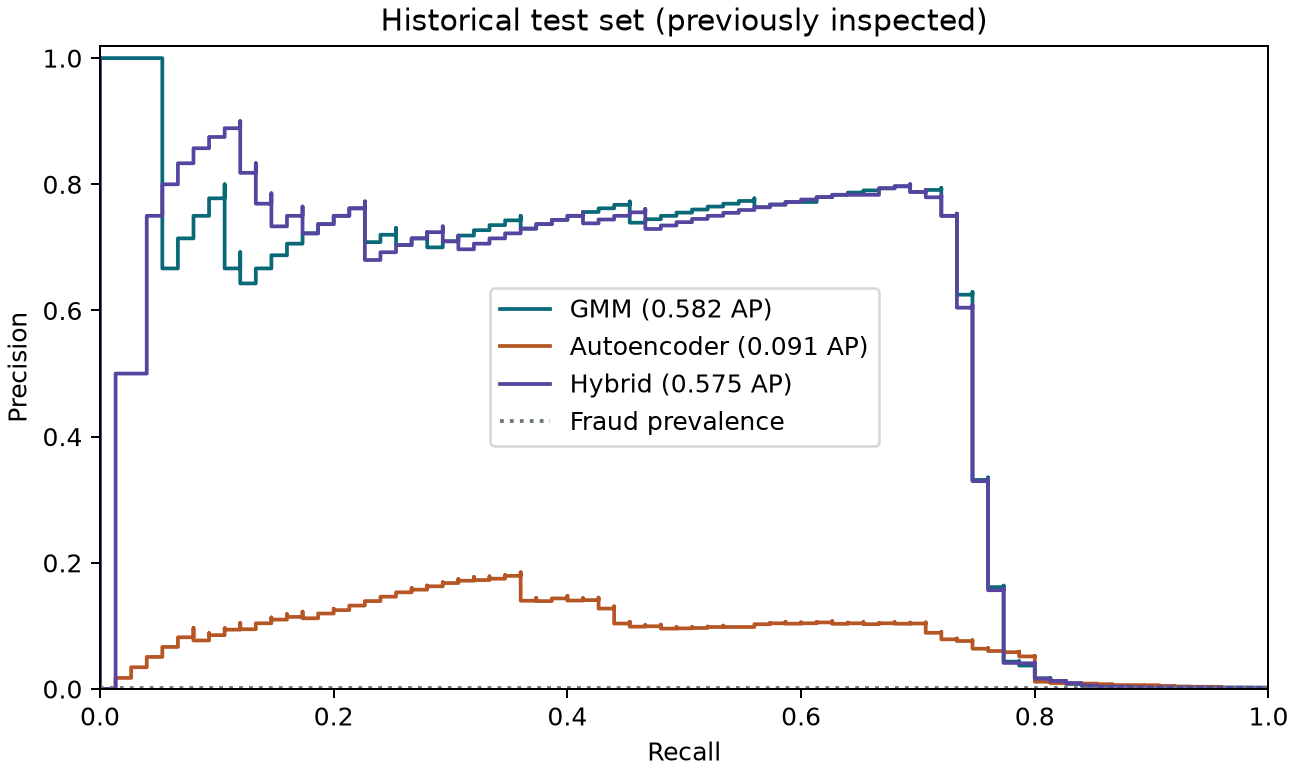
\includegraphics[width=\columnwidth]{test_pr_hybrid.png}
\caption{Hybrid and standalone precision-recall curves on the previously inspected historical test.}
\label{fig:hybrid}
\end{figure}

The hybrid modestly raises validation AP. On the historical test, its AP is lower and its fraud counts at each tested review capacity match GMM. At the 1\% validation FPR budget, both catch 58 frauds and the hybrid produces 320 false alerts versus 324 for GMM. The descriptive 95\% interval for the paired historical AP difference on 300 class-stratified bootstrap samples is $[-0.0437,0.0443]$. The small workload difference does not establish a reliable advantage. The hybrid notebook provides all budgets, capacities and validation weights.

\section{Limitations and Reproducibility}
The data cover two historical days and the PCA representation limits business-level explanations. The historical test partition was previously inspected. Confirmation requires unseen, compatible transactions and decisions frozen before scoring. The ablations used mixed validation only. The bootstrap conditions on the class counts and fitted scores and does not model temporal dependence.

Run \texttt{run\_phase2\_study.py} and \texttt{run\_phase2\_hybrid.py} with the original CSV to regenerate the studies. They verify split membership and record input hashes and configuration. Both notebooks read recorded outputs so reviewers can execute them without the raw CSV.

\begin{thebibliography}{6}
\bibitem{dempster} A. P. Dempster, N. M. Laird, and D. B. Rubin, Maximum likelihood from incomplete data via the EM algorithm, \emph{J. Roy. Stat. Soc. B}, vol. 39, no. 1, pp. 1--38, 1977.
\bibitem{sakurada} M. Sakurada and T. Yairi, Anomaly detection using autoencoders with nonlinear dimensionality reduction, in \emph{Proc. MLSDA}, pp. 4--11, 2014.
\bibitem{vincent} P. Vincent et al., Stacked denoising autoencoders: Learning useful representations in a deep network with a local denoising criterion, \emph{J. Mach. Learn. Res.}, vol. 11, pp. 3371--3408, 2010.
\bibitem{saito} T. Saito and M. Rehmsmeier, The precision-recall plot is more informative than the ROC plot when evaluating binary classifiers on imbalanced datasets, \emph{PLOS ONE}, vol. 10, no. 3, 2015.
\bibitem{ulb} ULB Machine Learning Group, Credit Card Fraud Detection. \url{https://www.kaggle.com/datasets/mlg-ulb/creditcardfraud}
\bibitem{sklearn} Scikit-learn, MLPRegressor. \url{https://scikit-learn.org/stable/modules/generated/sklearn.neural_network.MLPRegressor.html}
\end{thebibliography}
\end{document}
